\chapter{To-be named Chapter}
\label{sec:implementation}

\section{Study Area}
The study area encompasses the geographic mainland region of Portugal, extending 89,000 km\textsuperscript{2} located between latitude 42.3°N to 36.7°N and longitude 9.8°W to 6.0°W. Portugal experiences a Mediterranean climate influenced by the Atlantic Ocean and characterized by a mostly wet and cool season followed by a dry summer \cite{Mora2020, portugalClimate01, Marques2011}.

Altitudes range from sea level to  2000 metres, and higher elevations are more prevelent central and northern regions \cite{Marques2011}.

The northern region is characterised by lower temperatures and higher values of precipitation than the southern region \cite{Marques2011}. The average annual temperature ranges from 7 to 18°C, while the annual rainfall ranges from 400 to 2,800 mm.

Portugal's vegetation is a blend of Atlantic, European, Mediterranean, and African species \cite{britannica_portugal_climate}, and four tree species account for 80\% of all the forest area: \textit{Pinus pinaster}, \textit{Eucalyptus globulus}, \textit{Quercus suber}, and \textit{Quercus rotundifolia} \cite{Marques2011}.





\section{Dataset Sources}

\subsection{Wildfire Occurrences}
Historical records of fire occurrences were taken from \cite{centraldedados_incendios_website, centraldedados_incendios} and \cite{icnf2024}. The records featured in \cite{centraldedados_incendios_website, centraldedados_incendios} span across 35 years, from 1980 to 2015, and hold 791453 instances of wildfires. Its most relevant features are encapsulated in table \ref{historical_occurrences_1980_2015}, and table \ref{number_occurrences_1980_2013} holds the fire records for each year.


The records from \cite{icnf2024} span across 10 years, from 2013 to 2023, and were retrieved with an API \href{https://fogos.icnf.pt/localizador/webserviceocorrencias.asp?ano=YEAR}{endpoint}. It features 140514 entries, and its most important fields are described in table \ref{number_occurrences_1980_2013}, while table \ref{number_occurrences_2013_2023} holds the number of occurrences individually by year.

\begin{table}[H]
	\caption{Field description of Historical fires from 1980 to 2015 \cite{centraldedados_incendios_website, centraldedados_incendios}}
	\label{historical_occurrences_1980_2015}
	\centering
	\small
	\begin{tabular}{cp{7.5cm}} % Adjust width as necessary
		\hline
		\textbf{Variable} & \textbf{Description}\\
		\hline
		ano  & Year of fire occurrence \\
		codigo\_sgif & Unique identifier for the fire occurrence \\
		tipo  & Kind of wildfire. The available options are: forest, slash-and-burn, false alarm, and agricultural.\\
		distrito  & District of fire occurrence. \\
		concelho  & Municipality of fire occurrence. \\
		freguesia  & Parish of fire occurrence.\\
		local  & Location of fire occurrence. \\
		ine  & Not described or explained anywhere. \\
		x | y  & Wildfire location. \\
		data\_alerta  & Wildfire warning date. \\
		hora\_alerta  & Wildfire warning hour. \\
		data\_extincao & Wildfire complete extinguishment date. \\
		hora\_extincao & Hour of wildfire complete extinguishment. \\
		data\_primeira\_intervencao & Date of first fire intervention \\
		hora\_primeira\_intervencao & Hour of first fire intervention \\
		fonte\_alerta & Authority or group of people who reported the fire first. \\
		nut & A Unique identifier for a given nomenclature of territorial units for statistics. \\
		area\_povoamento & Burnt settlement area. \\
		area\_mato & Burnt bush area.  \\
		area\_agricola & Burnt agricultural area. \\
		area\_pov\_mato & Sum of burned area from the burnt settlement area and burnt agricultural area.\\
		area\_total & Total burnt area. \\
		reacendimento & Describes if a given fire is a re-ignition from a previous wildfire. \\
		queimada & Identifies if a fire is a slash-and-burn. \\
		falso\_alarme & Identifies if it is a false alarm. \\
		fogacho & Identifies if it is a specific type of fire named a blaze. \\
		incendio & Identifies if it is a fire. \\
		causa & Numerical identifier for the fire cause. \\
		tipo\_causa & Description of fire cause. The available options are unknown, deliberate, natural, negligent fire, and undefined. \\
		\hline
	\end{tabular}
\end{table}


\begin{table}[H]
	\caption{Number of Fire occurrences between 1980 and 2015}
	\label{number_occurrences_1980_2013}
	\centering
	\begin{tabular}{lc}
		\hline
		Year & \multicolumn{1}{l}{Number of Occurrences} \\ \hline
		1980 & 2346                                      \\
		1981 & 6727                                      \\
		1982 & 3625                                      \\
		1983 & 4536                                      \\
		1984 & 7355                                      \\
		1985 & 8439                                      \\
		1986 & 5036                                      \\
		1987 & 7703                                      \\
		1988 & 6130                                      \\
		1989 & 21895                                     \\
		1990 & 10743                                     \\
		1991 & 14327                                     \\
		1992 & 14951                                     \\
		1993 & 14799                                     \\
		1994 & 19983                                     \\
		1995 & 31116                                     \\
		1996 & 28626                                     \\
		1997 & 23494                                     \\
		1998 & 34675                                     \\
		1999 & 25473                                     \\
		2000 & 34107                                     \\
		2001 & 31582                                     \\
		2002 & 33697                                     \\
		2003 & 30345                                     \\
		2004 & 34722                                     \\
		2005 & 50364                                     \\
		2006 & 31445                                     \\
		2007 & 31122                                     \\
		2008 & 23139                                     \\
		2009 & 34979                                     \\
		2010 & 32357                                     \\
		2011 & 35941                                     \\
		2012 & 30740                                     \\
		2013 & 27372                                     \\
		2014 & 11387                                     \\
		2015 & 23175                                     \\ \hline
		Total & 791453                                   \\
		\hline
	\end{tabular}
\end{table}


\begin{table}[H]
	\caption{Field description of Historical fires from 2013 to 2023 \cite{icnf2024}}
	\label{historical_occurrences_2013_2023}
	\centering
	\small
	\begin{tabular}{cp{8.5cm}}
		\hline
		\textbf{Variable} & \textbf{Description}\\
		\hline
		CODIGO id  & Unique identifier for the fire occurrence \\
		DISTRITO  & District of fire occurrence. \\
		TIPO  & Kind of wildfire. The available options are: forest and agricultural fire.\\
		ANO  & Year of fire occurrence \\
		AREAPOV & Burnt settlement area. \\
		AREAMATO & Burnt bush area.  \\
		AREAAGRIC & Burnt agricultural area. \\
		AREATOTAL & Total burnt area. \\
		REACENDIMENTOS & Boolean value for reignition. \\
		FOGACHO & Boolean value for small fire. \\
		Incendio & Boolean value for fire. \\
		Agricola & Boolean value for agricultural fire. \\
		DATAALERTA & Wildfire warning date. \\
		HORAALERTA & Wildfire warning hour. \\
		LOCAL & Location of fire occurrence \\
		CONCELHO & Municipality of fire occurrence. \\
		FREGUESIA & Parish of fire occurrence\\
		FONTEALERTA & Authority or group of people who reported the fire first. \\
		DIA & Day of the fire occurrence. \\
		MES & Month of fire occurrence. \\
		HORA & Fire hour of occurrence. \\
		CAUSA & Numerical identifier for the fire cause. \\
		TIPOCAUSA & Description of fire cause. The available options differ from year to year. \\
		DHINICIO & Firefighting starting date and time \\
		DHFIM & Ending of firefighting efforts\\
		DURACAO & Number of minutes it took to extinguish the fire \\
		HAHORA & Not described \\
		DATAEXTINCAO & Fire extinguish date \\
		HORAEXTINCAO & Fire extinguish hour \\
		QUEIMA & Boolean value for intentional small fire\\
		LAT & Latitude coordinate of fire occurrence\\
		LON & Longitude coordinate of fire occurrence\\
		TEMPERATURA & Value for temperature at the time of fire occurrence\\
		HUMIDADERELATIVA & Relative Humidity value\\
		VENTOINTENSIDADE & Wind velocity\\
		VENTODIRECAO\_VETOR & Direction of wind\\
		PRECIPITACAO & Value for rainfall\\
		FFMC & Fine fuel moisture code\\
		DMC & Duff moisture code\\
		DC & Drought code\\
		ISI & Initial Spread index\\
		BUI & Build Up Index\\
		FWI & Fire Weather Index\\
		DSR & Daily Severity Rating\\
		ALTITUDEMEDIA & Mean altitude\\
		DECLIVEMEDIO & Mean Slope\\
		\hline
	\end{tabular}
\end{table}

\begin{table}[H]
	\centering
	\caption{Number of Fire occurrences between 2013 and 2023}
	\label{number_occurrences_2013_2023}
	\begin{tabular}{lc}
		Year  & \multicolumn{1}{l}{Number of Occurrences} \\ \hline
		2013  & 24479                                     \\
		2014  & 10286                                     \\
		2015  & 19669                                     \\
		2016  & 16131                                     \\
		2017  & 21074                                     \\
		2018  & 12296                                     \\
		2019  & 10909                                     \\
		2020  & 9713                                      \\
		2021  & 6996                                      \\
		2022  & 1335                                      \\
		2023  & 7626                                      \\ \hline
		Total & 140514                                    \\ \hline
	\end{tabular}
\end{table}



\subsection{Weather Variables}
Historical weather variables were obtained via the \textit{Open-Meteo API} \cite{Zippenfenig_Open-Meteo}. Which includes daily and hourly weather data extraction from all across the world. The API compares the provided location to several reanalysis datasets and returns the most optimal result based on location. It includes a full database of historical hourly weather conditions dating back to 1940 from multiple sources (table \ref{Datasets_api}). 

The API incorporates observations from weather stations, aeroplanes, buoys, radar, and satellites and it fills gaps in data using mathematical models to estimate the values of different weather variables \cite{Zippenfenig_Open-Meteo}.


The variables extracted from \textit{Open-Meteo} are on table \ref{open_meteo_variables} as well as the unit for each weather variable.


\begin{table}[H]
	\caption{API Weather Sources \cite{Zippenfenig_Open-Meteo, Hersbach_ERA5, Munoz_ERA5_LAND, Schimanke_CERRA}}
	\centering
	\label{Datasets_api}
	\begin{tabular}{llll}
		\hline
		\multicolumn{1}{c}{Dataset} & \multicolumn{1}{c}{Region} & \multicolumn{1}{c}{Resolution} & \multicolumn{1}{c}{Availability} \\ \hline
		ECMFWF IFS & Global & 9km, Hourly  & 2017 to present   \\
		ERA5       & Global & 25km, Hourly & 1940 to present   \\
		ERA5-Land  & Global & 11km, Hourly & 1950 to present   \\
		CERRA      & Europe & 5km, Hourly  & 1985 to June 2021
	\end{tabular}
\end{table}




\begin{table}[H]
	\caption{Hourly weather variables from \textit{Open-meteo}}
	\centering
	\small
	\label{open_meteo_variables}
	\begin{tabular}{ccp{10cm}} % Adjust width as necessary
		\hline
		\textbf{Variable} & \textbf{Unit} & \textbf{Description}\\
		\hline
		Temperature & °C & Air temperature 2 metres above ground. \\
		\hline
		Relative Humidity & \% & Relative humidity 2 metres above ground. \\
		\hline
		Dew & °C & Dew point 2 metres above ground. \\
		\hline
		Apparent Temperature & °C & Apparent temperature is the 
		result of a wind chill factor, relative humidity, and solar radiation. \\
		\hline
		Pressure & hPa & Atmospheric air pressure reduced to mean sea level. \\
		\hline
		Surface Pressure & hPa & Surface pressure reduced to mean sea level. \\
		\hline
		Precipitation & mm & Sum of preceding hour precipitation including rain, showers, and snow. \\
		\hline
		Rain & mm & Preceding hour of liquid precipitation. \\
		\hline
		Snowfall & cm & Preceding hour of snowfall amount. \\
		\hline
		Cloud cover low & \% & Fog and low level clouds up to an altitude of 2 kilometres. \\
		\hline
		Cloud cover mid & \% & Clouds floating at a medium level with altitudes ranging from 2 kilometres to six kilometres. \\
		\hline
		Cloud cover high & \% & Clouds floating at an altitude of 6 kilometres. \\
		\hline
		Shortwave radiation & $W/m^2$ & Shortwave solar radiation.  \\
		\hline
		Direct radiation & $W/m^2$ & Direct solar radiation. \\
		\hline
		Direct normal irradiance & $W/m^2$ & Direct solar irradiance.  \\
		\hline
		Diffuse radiation & $W/m^2$ & Diffuse solar radiation.  \\
		\hline
		Global tilted irradiance & $W/m^2$ & Total radiation received on a tilted pane.  \\
		\hline
		Sunshine duration & Seconds & Duration of sunshine in seconds.  \\
		\hline
		Wind speed at 10m & km/h & Speed of the wind, 10 metres above ground.  \\
		\hline
		Wind speed at 100m & km/h & Speed of the wind, 100 metres above ground.  \\
		\hline
		Wind direction at 10m & ° & Wind direction at 10 metres above ground.  \\
		\hline
		Wind direction at 100m & ° & Wind direction at 100 metres above ground.  \\
		\hline
		Wind gusts & km/h & Wind gusts at 10 metres above ground.  \\
		\hline
		Evapotranspiration & mm & Evapotranspiration value for the required irrigation for plants calculated from temperature, wind speed, humidity, and solar radiation. \\
		\hline
		Weather code & WMO code & Numeric codes for weather conditions.  \\
		\hline
		Snow depth & meters & The depth of snow on the ground.  \\
		\hline
		Vapour pressure deficit & kPa & Vapour pressure deficit in kilopascal.\\
		\hline
		Soil temperature & °C & Average soil temperature ranging from 0 to 7cm, 7 to 28cm, 28 to 100cm, and 100 to 255cm below ground.\\
		\hline
		Soil moisture & $m^3/m^3$ & Average soil moisture ranging from 0 to 7cm, 7 to 28cm, 28 to 100cm, and 100 to 255cm depths.\\
		\hline
	\end{tabular}
\end{table}







\subsection{Fuel Variables}
Fuel variables encompass two sources: Copernicus Climate Change Service \cite{CopernicusCDS2019} and Forestry Inventory 2015 \cite{uva2021forestry,https://doi.org/10.15468/dl.zwfmbt}

\subsubsection{Copernicus Climate Change Service \cite{CopernicusCDS2019}}

The Copernicus Climate Change Service contains daily historical reconstructions of fire danger indices, i.e., variables that emphasize conditions suitable for the origin, spread, and sustainability of naturally occurring fires. The fire danger indices are obtained from historical simulations and weather forecasts, and the available data starts in January 1940 and extends all the way through 2023. Variables contained in the dataset are expressed in the table \ref{copernicus_danger_indices}.
From this source, all variables that belong to the fire weather index system were extracted except the fire daily severity index, which is not necessary for the calculation of fwi.

\begin{table}[H]
	\caption{Fire danger indices from historical data \cite{CopernicusCDS2019}}
	\label{copernicus_danger_indices}
	\centering
	\small
	\begin{tabular}{ccp{7.5cm}} % Adjust width as necessary
		\hline
		\textbf{Variable} & \textbf{Unit} & \textbf{Description}\\
		\hline
		Build-up index & Dimensionless & Weighted combination of the Duff moisture code and Drought code. \\
		\hline
		Drought code & Dimensionless & Component representing fuel availability, and the influence of recent temperatures and rainfall events on fuel availability. \\
		\hline
		Duff moisture code & Dimensionless & Moisture content in loosely-compacted organic layers of moderate depth. Duff moisture code fuels are affected by rain, temperature and relative humidity. \\
		\hline
		Fine fuel moisture code & Dimensionless &  Moisture content in litter. Representative of the top litter layer less than 1-2 cm deep. \\
		\hline
		Fire daily severity index & Dimensionless &  A numerical assessment of the difficulty of controlling flames. \\
		\hline
		Fire weather index & Dimensionless &  Combination of Initial spread index and Build-up index. Numerical rating of the potential fire intensity. \\
		\hline
		Initial spread index & Dimensionless & Combines fine fuel moisture code with weed speed to measure the expected rate of fire spread.
	\end{tabular}
\end{table}

\subsubsection{Forestry Inventory 2015 \cite{uva2021forestry,https://doi.org/10.15468/dl.zwfmbt}}

The Forestry Inventory 2015 contains 579422 occurrences of forest tree species on mainland Portugal. The data was gathered using aerial images and ground surveys. The most important features of the dataset are described in Table \ref{forest_inventory}. From this source, the only variable taken was the name of the tree species closest to the wildfire area.

\begin{table}[H]
	\caption{Forest Inventory 2015}
	\label{forest_inventory}
	\centering
	\small
	\begin{tabular}{cp{7.5cm}} % Adjust width as necessary
		\hline
		\textbf{Variable} & \textbf{Description}\\
		\hline
		gbifID | datasetKey | ocurrenceID  & Identifiers for the occurrence of trees and the dataset. \\
		kingdom & Kingdom classification of a given Tree. \\
		phylum & Phylum classification of a given Tree. \\
		class & Taxonomic class. \\
		order & Taxonomic Order of a Tree. \\
		genus & Tree genus. \\
		species & Data containing the species of a given tree. \\
		taxonRank & Data containing the highest taxonomic rank available for a given tree group. \\
		scientificName | verbatimScientificName & Scientific name for the available taxonomic classification. \\
		
		verbatimScientificNameAuthorship & Scientific name authorship for the available taxonomic classification. \\
		
		countryCode & Contry code of Portugal. \\
		
		locality & Name of a locality containing a given tree. \\
		
		stateProvince &  Name of a district containing a given tree. \\
		
		occurrenceStatus & Describes if a tree is still present.   \\
		
		decimalLatitude & Latitude for the tree occurrence. \\
		
		decimalLongitude & Longitude for the tree occurrence \\
		
		coordinateUncertaintyInMeters & Uncertainty for a given tree location in metres. \\
		
		eventDate | year & Year of event record. \\
		
		taxonKey & Taxonomic key for the highest available classification for a tree \\
		
		speciesKey & Individual key for a given tree species if available. \\
		
		speciesKey & Individual key for a given tree species if available. \\
		
		institutionCode & Unique identifier for ICNF. \\
		
		collectionCode & Unique collection identifier for the institutionCode. \\
	\end{tabular}
\end{table}


\subsection{Topography Variables}
Topography includes data from three distinct sources. The mean elevation was taken from GMTED2010 \cite{Danielson2011}. The land class type was extracted from Corine Land Cover \cite{71c95a07-e296-44fc-b22b-415f42acfdf0}, and the slope, aspect, and roughness were extracted from GLO-30 \cite{ESA_Sinergise_2021}.

\subsubsection{Global Multi-Resolution Terrain Elevation Data 2010 \cite{Danielson2011}}
GMTED2010 is a source that provides raster elevation data. For every wildfire location, the mean elevation was extracted with a resolution of 7.5 arcseconds. 

\subsubsection{Corine Land Cover \cite{71c95a07-e296-44fc-b22b-415f42acfdf0}}
Corine Land Cover is a dataset that provides European land classification from 44 thematic classes. From this source, the land class corresponding to the location of a wildfire event was extracted.

\subsubsection{Copernicus GLO-30 Digital Elevation Model \cite{ESA_Sinergise_2021}}
The GLO-30 Digital Elevation Model is a digital surface model. It encompasses the earth's surface with its buildings, infrastructure, and vegetation.

From this source, slope, aspect, and roughness were extracted with a resolution of 30 meters for every wildfire occurrence.


\subsection{Dataset variables}
All the variables used in the dataset are listed in Table \ref{other_variables}. 


\begin{table}[H]
	\centering
	\caption{Topography, Weather and Fuel variables}
	\label{other_variables}
	\begin{tabular}{ccc}
		\hline
		\textbf{Variable Type} & \textbf{Variable Name} & \textbf{Resolution} \\ \hline
		\multirow{4}{*}{Topography} & Mean Elevation (m) & \_,7.5 arc-seconds, \_ \\
		& Slope (0-90°) & 30m, \_, \_ \\
		& Roughness & 30m, \_, \_ \\
		& Aspect (0-360°) & 30m, \_, \_ \\ \hline
		Weather & 
		\begin{tabular}[c]{@{}c@{}}
			Temperature (°C)\\ 
			Relative Humidity (\%)\\ 
			Dew (°C)\\ 
			Apparent Temperature (°C)\\ 
			Pressure (hPa)\\ 
			Surface Pressure (hPa)\\ 
			Precipitation (mm)\\ 
			Rain (mm)\\ 
			Snowfall (cm)\\ 
			Cloud Cover Low/Mid/High (\%)\\ 
			Shortwave Radiation ($W/m^2$)\\ 
			Direct Radiation ($W/m^2$)\\ 
			Direct Normal Irradiance ($W/m^2$)\\ 
			Diffuse Radiation ($W/m^2$)\\ 
			Global Tilted Irradiance ($W/m^2$)\\ 
			Sunshine Duration (Seconds)\\ 
			Wind Speed 10m/100m (km/h)\\ 
			Wind Direction 10m/100m (°)\\ 
			Wind Gusts 10m (km/h)\\ 
			Et0 Evapotranspiration (mm)\\ 
			Weather Code (WMO code)\\ 
			Snow Depth (metres)\\ 
			Vapour Pressure Deficit (kPa)\\ 
			Soil Temperature 0 to 255cm (°C)\\ 
			Soil Moisture 0 to 255cm ($m^3/m^3$)
		\end{tabular} & 
		0.25/0.1/9km/5km, \_ , Hourly \\ \hline
		Fuel & 
		\begin{tabular}[c]{@{}c@{}}
			Fine fuel moisture code\\ 
			Duff moisture code\\ 
			Drought code\\ 
			Initial Spread index \\ 
			Build Up Index \\ 
			Fire weather index\\ 
			Tree Species
		\end{tabular} & 
		\begin{tabular}[c]{@{}c@{}}
			0.25 , \_ , Daily\\ \\ \\ \\ \\ -
		\end{tabular} \\ \hline
	\end{tabular}
\end{table}


\subsection{Additional sources of Data}
The python library geopy \cite{geopy} was used to geolocate multiple locations, resolving district, parish, municipalities, and localities to sets of coordinates. Geopy utilises multiple geocoding web services like OpenStreetMap Nominatim and Google Geocoding API to resolve locations. 


The Google Maps service \cite{googlexmaps} was used to manually check if samples extracted from Open-Meteo corresponded to the intended location. It was also used to analyse some errors that were found in the location of some entries.


\section{Data Preparation of historical wildfire sites}
This section covers the time frame selected for study and the selection of wildfire ignition causes.


\subsection{Selecting the time frame of wildfire occurrences}

The dataset described in \ref{historical_occurrences_1980_2015} is composed of multiple files describing historical occurrences since 1980 until 2015. Prior to 2001, the fields from each file became unstandardized, and there's no explicit parameter mentioning a natural wildfire cause. Therefore, the time frame considered was from 2001 to 2012. The latter years were rejected due to the fact that entries from \ref{historical_occurrences_1980_2015} do not contain any explicit latitude and longitude. They rely on territorial entities such as districts, municipalities, parishes, and NUTS to describe locations.

The second historical wildfire dataset \ref{historical_occurrences_2013_2023} is also composed of multiple files. Its time frame is from 2013 until 2023. Unlike dataset \ref{historical_occurrences_1980_2015}, entries do contain an explicit latitude and longitude values. It also features descriptive territorial entities. 

\subsection{Ignition cause selection}
Historical wildfire sites whose cause was set as deliberate or negligent fire were excluded. The remaining causes left in the dataset, in order of importance, are: natural, reignition, unknown, and undefined. For the creation of the first dataset, all these causes were encompassed. The undefined cause differed from the unknown cause due to the fact that their cause field was left blank, and entries that had unknown causes were explicitly described as unknown. Since the remaining causes aren't an object of study and their importance relies solely on inventory, their analysis won't be assessed in this thesis. Table \ref{tab:incidents_fires} contrasts reignition, unknown, and undefined causes with only natural causes. It is possible to observe that fires whose cause is set as natural have a tiny proportion compared to the outside scope of unknown, undefined, and reigniting causes of ignition. The undefined causes were labeled as \textit{NC} (as for non-characterised) in the dataset.



\begin{table}[H]
	\centering
	\caption{Proportion of natural fires compared to other causes from 2001 to 2023}
	\label{tab:incidents_fires}
	\begin{tabular}{lrr}
		\toprule
		Year & Reignition | Unknown | Undefined & Natural Fires \\
		\midrule
		2001 & 25938 & 44 \\
		2002 & 25637 & 13 \\
		2003 & 25042 & 96 \\
		2004 & 21173 & 16 \\
		2005 & 34575 & 3 \\
		2006 & 19108 & 67 \\
		2007 & 15565 & 50 \\
		2008 & 9877  & 28 \\
		2009 & 17293 & 106 \\
		2010 & 14293 & 138 \\
		2011 & 14811 & 102 \\
		2012 & 11785 & 56 \\
		2013 & 11822 & 77 \\
		2014 & 3795  & 38 \\
		2015 & 8293  & 138 \\
		2016 & 7715  & 67 \\
		2017 & 10308 & 104 \\
		2018 & 5445  & 114 \\
		2019 & 3912  & 128 \\
		2020 & 3858  & 95 \\
		2021 & 2507  & 103 \\
		2022 & 3925  & 115 \\
		2023 & 2427  & 72 \\
		\midrule
		TOTAL & 299104 & 1770 \\
		\bottomrule
	\end{tabular}
	
\end{table}

\section{Historical Meteorological Data Extraction}

\subsection{Retrieving historical meteorological data}
Extracting historical meteorological data for the dataset described in \ref{historical_occurrences_2013_2023} was done with ease with a Python script. It went through each historical fire location and downloaded hourly weather data about the entire day regarding the wildfire occurrence. For each wildfire site, a file was created with the date of the occurrence and fire coordinates. All files followed this convention. A latter approach dismissed this method of individually creating files for each site as it proved to be less efficient than having multiple sites in one batch of occurrences (further explanation on this topic will be featured in section \ref{Natural_Fires_dataset}, which covers the creation of the natural fires dataset). 


As for the dataset in \ref{historical_occurrences_1980_2015}, it was necessary to geocode the position of each occurrence individually. For both datasets, all the variables described in table \ref{open_meteo_variables} were extracted.

\subsection{Geocoding places from 2001 to 2012 historical wildfire locations}
\label{geocoding_historical}
The dataset entries featured in \ref{historical_occurrences_1980_2015} contain no direct field leading up to the real site location coordinates. To tackle this issue, an algorithm with the help of the geopy library \cite{geopy} was made to resolve the names of historial wildfire places to a set of coordinates. It was necessary to try multiple combinations to obtain the best results (see table \ref{geocoding_entries_2001_2012} for the list of combinations), since the services provided by the geopy library aren't as robust as \textit{Google Maps}. The district, municipality, parish, and local (if available) of each entry were utilized for the purpose of geocoding. Sometimes, the name of the exact wildfire locality was enclosed in brackets, requiring processing using strings to extract it.


\begin{table}[H]
	\caption{Combinations for local geocoding}
	\label{geocoding_entries_2001_2012}
	\centering
	\small
	\begin{tabular}{cp{7.5cm}|}
		\hline
		\textbf{Combination}\\
		\hline
		Local, District\\
		\hline
		Local, Parish, District\\
		\hline
		Local, Parish, Municipality\\
		\hline
		Local, Parish, Municipality, District\\
		\hline
		Parish, Municipality, District\\
		\hline
		Local, Parish, District\\
		\hline
	\end{tabular}
\end{table}


These combinations caused errors in the location of some entries because the geocoders returned coordinates in other countries, such as Spain and Brazil, due to similar names in some locations. The entries that produced errors underwent recalculation, with the addition of "Portugal" at the end. An example of this usage is  {\it Parish, District, Portugal}.

After each entry was resolved, their latitude and longitude were added as values in the columns \textit{LAT} and \textit{LON} of each corresponding wildfire site in the file containing the historical wildfire data.


A very minor sample of entries couldn't be geocoded using this method. Therefore they were manually geocoded from the \textit{Google Maps} service. 



\section{Crafting the First dataset}
\label{the_first_dataset}
At this point, wildfire sites from the source \ref{historical_occurrences_1980_2015} were geocoded, and the weather data corresponding to the day of occurrence for each wildfire was extracted. It was now necessary to go through each downloaded file and extract the most relevant attributes. Each file contained attributes that were not necessary to explain the problem of fires. 


For example, the variables had a separate column with their respective units. Columns that featured units were dropped. The rest of the columns that were not considered were: \textit{latitude and longitude} (these coordinates refer to the weather station location and not to the wildfire site), \textit{generationtime\_ms, utc\_offset\_seconds, timezone,} and \textit{timezone\_abbreviation}. 

These methods were conducted repeatedly each year. At this stage, each year had a separate file with its historical wildfire sites, and the dataset had the following variables: \textit{year, date, district, municipality, parish, local, latitude, longitude, cause, elevation} (this variable comes with the weather data, but since it is not optionally chosen, it hasn't been mentioned before) plus all the weather variables from \textit{Open-Meteo} (table \ref{open_meteo_variables}).


After extracting the weather data for the day of each wildfire occurrence, it was time to match each site with the surrounding tree species. 



\subsection{Matching historical wildfire with tree species}
\label{tree_species_wildfires}

In order to match each fire event with the surrounding tree species, it was necessary to separate the events by district. Within each district, the parish or municipality of each occurrence was matched with the parish or municipality of the tree species. For instances without a match within the district, they were matched with a distance function named \textit{Haversine}, which is a method for calculating the distance between two locations on a sphere's surface based on their latitude and longitude \cite{esri2024}. This function calculated the distance between the coordinates of the wildfire event and the coordinates of each tree species location. 


The distance calculation featured multiple tests. Experiments were done with 120, 500, and 1000 metres. The first distance threshold resulted in a lot of entries without a match. The distance threshold was slightly increased from 500 metres to 1000 metres, due to the fact that the latter distance was able to perform a match with the majority of wildfire events. Species that were in the same parish or municipality as the fire incident were associated without calculating distance. To combat duplicate species, a tree species was only added if it was not already contained in the fire entry.

For the remaining entries that did not match the previous methods, an analysis was made of the species that were closest. In this step, errors were detected, some values tabulated by the ICNF did not correspond to reality, and some values in \ref{geocoding_historical} were miscalculated.


The forest inventory data source also contained some errors that had to be assessed. For instance, it wrongly stated a locality with a different name from its real-life counterpart. The locality \textit{Ovadas e Panchora} doesn't exist. It was misspelt, and its name is \textit{Ovadas e Panchorra}.


Other minor adjustments were also made. For example, each district had the word \textit{District} associated with its district name, like in \textit{Bragança District}, and the string \textit{District} was dropped to ensure standardisation between fire incidents and tree species.

Due to the size of the tree dataset, the Python script divided the years into chunks and used multiprocessing to calculate the tree species near the wildfire event.



\subsection{Locations in the middle of the sea.}
Between 2013 and 2023, some of the featured locations provided by the \textit{ICNF} were in the middle of the ocean. Although using their district, municipality, parish, or local field when using services like \textit{Google Maps} yielded in a real-life location. Their coordinates were undeniably wrong, since they were kilometres away from the nearest coast line. For these entries, weather extraction and tree species matching were redone. 


These multiple geolocation errors were discovered when trying to pin multiple species of trees (\ref{tree_species_wildfires}) to a single location with the distance function calculator. The algorithm returned values that were outside of the range spectrum previously set at 1000 metres. Leading up to the manual confirmation of these errors with the help of the \textit{Google Maps service}.


\subsection{Dataset description - Falta acabar}
The dataset features 300874 entries. 

number of entries of each type 300874
1770 natural
64207 Desconhecida Unknown
222596 NC undefined
12301 Reigniton



This dataset does not contain any topographical data and fuel data, except for the surrouding tree species, corresponding to the location of the fires. It only features weather variables at the hour the fire ignited. Although the object of study is fires of natural origin, this dataset was created in order to have a historical reference for fires that occurred between 2001 and 2023 and whose cause could not be ascertained. So that in the future it would be possible to determine the origin of fires of uncertain origin and characterise them. From this dataset, all wildfires whose origin was only natural were extracted.





\section{Natural Fires dataset}
\label{Natural_Fires_dataset}
The primary focus of the research is on naturally occurring fires. What has been done in relation to natural-origin fires is covered in this section. Fires whose cause was natural were taken out of the prior dataset with its weather records at the time of ignition and previously matched tree species. Making it 1770 natural-occurring fires. Another meteorological data extraction was done, this time encompassing a larger time frame. Then, a FWI calculation for the entries was performed, and each fire was then matched with the topographical data relating to its location.

\subsection{Weather history extraction for natural fires}
Instead of only gathering hourly weather history relative to the day of wildfire igniton. For natural fires, a total of 3 months of weather data prior to and during the ignition were extracted. It also featured hourly data, and the variables were the same as previously described in Table (\ref{open_meteo_variables}).
This time, instead of extracting each fire individually, batches were created to host 100 different fires per batch. Each batch held 3-month weather records for each fire. This proved to be faster for extracting and analysing. Still, each fire was split into an individual file containing only its weather records. This was done in order to save time, and it worked as a saving system for FWI calculation as it proved to be computationally expensive.
The same variables referenced in \ref{the_first_dataset}  were dropped aswell.

\subsection{FWI Calculation}
FWI is especially important because it can predict the risk of a wildfire by addressing the different fuels found in forest soils \cite{IPMA2024}. The source of data \ref{copernicus_danger_indices} contains daily data at 12:00 for fwi and the variables that compose it. However, for a further analysis of the topic, it is crucial to calculate the values of fwi and its variables for the remaining hours of the day. To ensure calculation accuracy, a Python library named \textit{pyfwi} \cite{buckinha2024} was used. The equations inside the library were compared to the official FWI guide \cite{van1985equations} to assure the calculations were being done correctly.
A comparison between the results from IPMA and the calculated FWI values was done. In the paper \cite{ipma2015}, the authors show a chart for FWI in the month of May of 2015 (right-side of image \ref{fig:comparison_fwi_ipma}). This chart encompasses the average daily values for 68 different weather stations. However, the appendix to the report didn't specify the weather stations used. Instead, it provided a list of 80 weather stations. Without the chance of getting to know the weather stations used, an experiment was conducted with all 80 stations. Firstly, weather data for the last days of April and the entire month of May for 2015 were extracted for every location set in the report. Then, the months of April and May 2015 were downloaded from \cite{CopernicusCDS2019}. The equations for FWI require starting values. Those were extracted from the tabulated values of the last days of April from the Copernicus source. For the entire month of May, tabulated values weren't used. Instead, each value was calculated with the \textit{pyfwi} library.
The results of this experiment are shown in image \ref{fig:comparison_fwi_ipma}. Even though the charts are not exactly the same, the underlying pattern remains the same, given the differences in the number of weather stations used in each example. Further comparisons between the continuous calculations of FWI and other sources will be assessed in the next chapter.

\begin{figure}[H]
	\caption{Comparison of average FWI calculated values and IPMA - 2015}
	\centering
	\begin{subfigure}{0.49\textwidth}
		\centering
		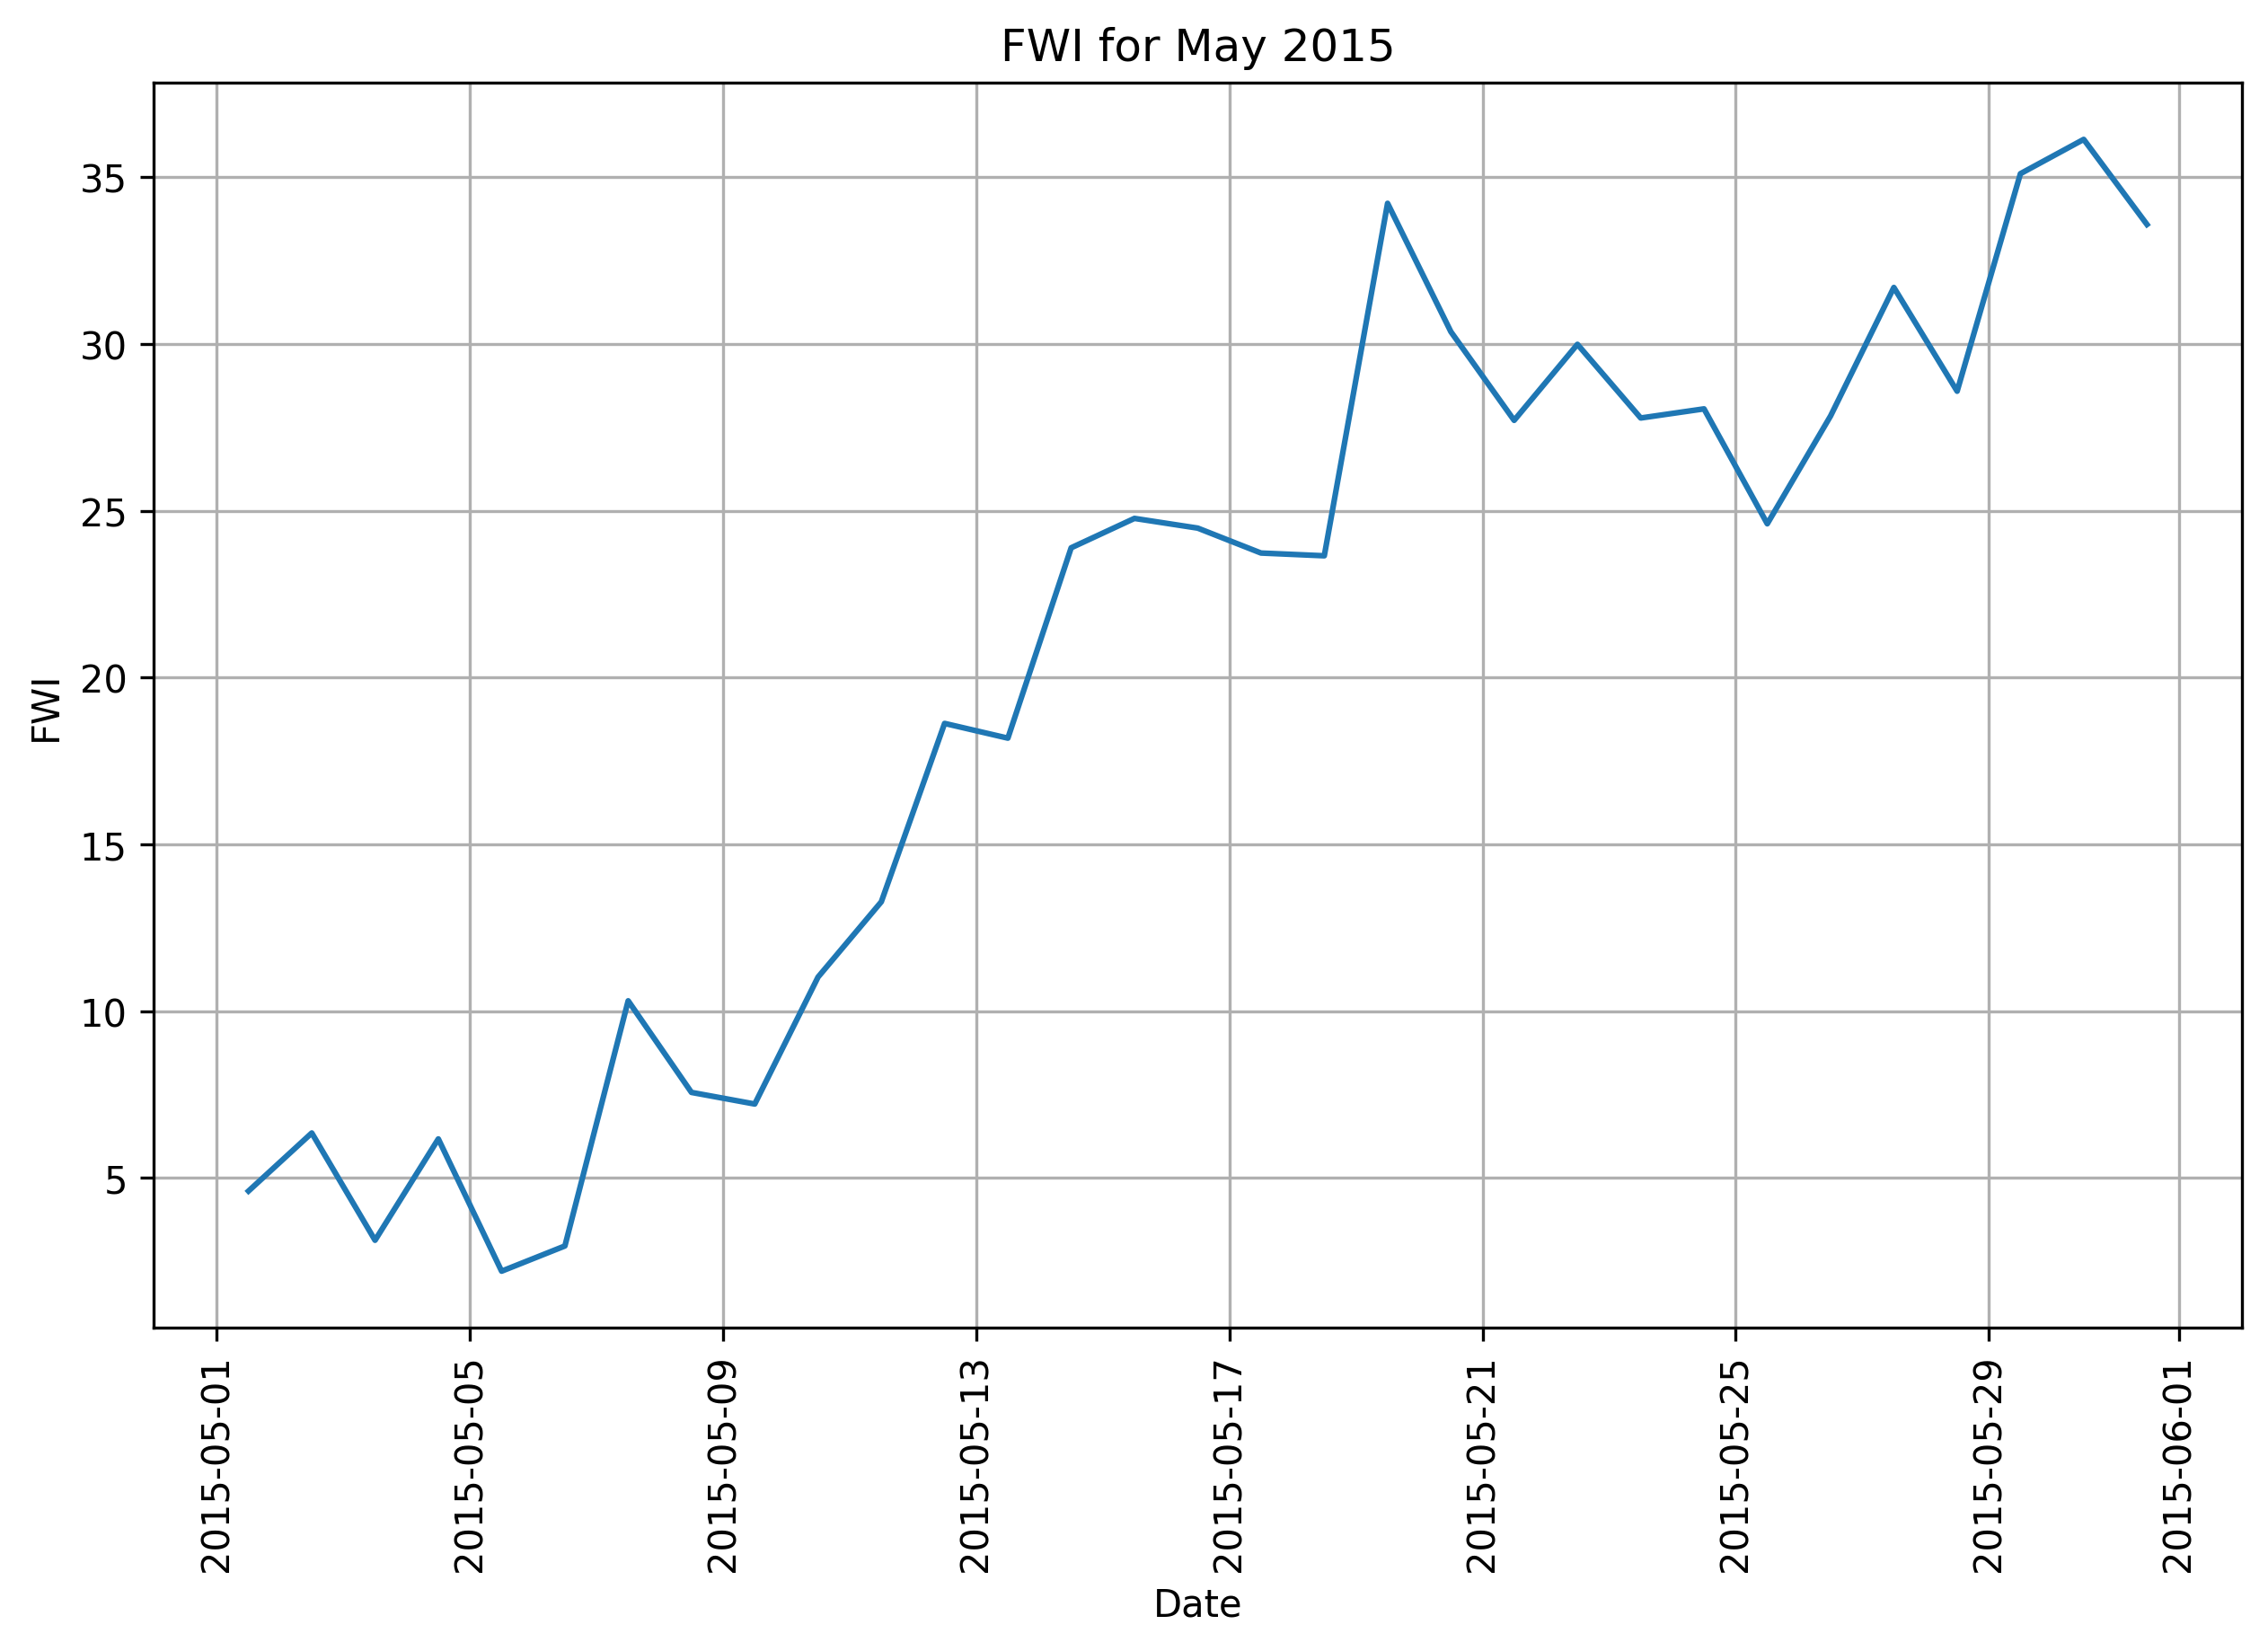
\includegraphics[width=\textwidth]{chapter-images/Datasetcreation/FWI/fwi_X1_plot.png}
		\caption{FWI - Calculated}
		\label{fig:fwi_copernicus_2022_midday}
	\end{subfigure}
	\hfill
	\begin{subfigure}{0.49\textwidth}
		\centering
		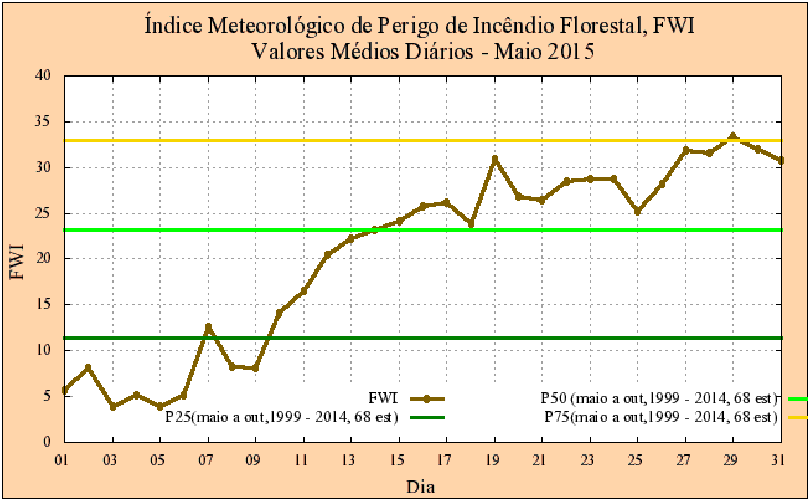
\includegraphics[width=\textwidth]{chapter-images/Datasetcreation/FWI/fwi_ipma.png}
		\caption{FWI - IPMA}
		\label{fig:fwi_calculated_2022_midday}
	\end{subfigure}
	\label{fig:comparison_fwi_ipma}
\end{figure}


For fires of natural origin, the same principles were applied. Every day at noon, the values were no longer calculated. The FWI equations require an initial value to work. The hourly FWI calculation worked in such a way that the initial values were those that were present in the previous hour. When the algorithm reached midday, it didn't use the values from the previous hour but the tabulated values from Copernicus. This method ensured that hours without a FWI tabulated value gained a value for FWI and all the variables necessary for it. This was conducted for each natural fire and for every hour of their 3-month weather history records.

Falta o algorithmo criado




\subsection{Creating Areas without wildfires}

Random Coordinates that were not equal to the ones in Natural Fires. A minimum distance of 25 km for each generated coordinated and the ones in Natural fires. With openstreet map given the range for latitude (36.7, 42.3) and longitude (-9.8, -6) check if the generated coordinate is in Portugal and check if it belongs to a county to ensure it isn't in the middle of the sea.








\subsection{Creating Areas without wildfires}

Random Coordinates that were not equal to the ones in Natural Fires. A minimum distance of 25 km for each generated coordinated and the ones in Natural fires. With openstreet map given the range for latitude (36.7, 42.3) and longitude (-9.8, -6) check if the generated coordinate is in Portugal and check if it belongs to a county to ensure it isn't in the middle of the sea.

\subsection{Dataset description}

%\begin{comment}
%\end{comment}






\section{Python libraries used in the conception of the dataset}
requests
pandas
os to check if files already existed.
numpy
sklearn



\section{Entry Selection}
Specifity how many entries raw files have.







\section{Models}


\subsection{Model Variables and their importance}

porque de escolher soil moisture 7 to 28cm e nao os outros gráfico de correspondencia.

temperature : 8
relative humidity: 8
precipitation': 16
wind speed: 16
soil temperature 28 to 100cm: 8
soil moisture 7 to 28cm: 8
direct normal irradiance: 8

'fwix': 8,
'ffmc': 8,
'dmc': 16,
'dc': 16,
'isi': 8,

roughness', 'aspect', 'slope', 'CLC CODE','scientificNames', 'mean elev'

tree species foram one hot encoded with MultiLabelBinarizer()

variables with multiple days were flattened

Slope has a significant influence on fire behaviour since it speeds its spread \cite{Marques2011}.


\subsection{Random Forest Classifier}



\subsubsection{Model with only Weather Variables}

Accuracy: 0.8248587570621468
Precision: 0.8532608695652174
Recall: 0.8177083333333334
F1 Score: 0.8351063829787234


\subsection{Model with weather and topography}

Accuracy: 0.9887005649717514
Precision: 0.9973544973544973
Recall: 0.9817708333333334
F1 Score: 0.989501312335958

\subsection{Model with weather, topography and fire weather}

Accuracy: 0.9830508474576272
Precision: 0.9946808510638298
Recall: 0.9739583333333334
F1 Score: 0.9842105263157894






